\chapter{実装}
本章では,本研究の実装環境をハードウェアとソフトウェアに分けて説明する.

\section{ハードウェアシステム構成}
本システムの構成を\figref{sys}に示す.本システムは主にHMD・VIVEトラッカー・PC・コントローラ―で構成される.被験者はHMDを装着した状態で右手にコントローラーを持つ.
ベースステーションでコントローラ―に取り付けられたVIVEトラッカーを読みとりPCに情報を送信する.その情報をにしたがい,仮想空間上に魔法の杖を表示しHMDに描画する.

\begin{figure}[h]
\centering
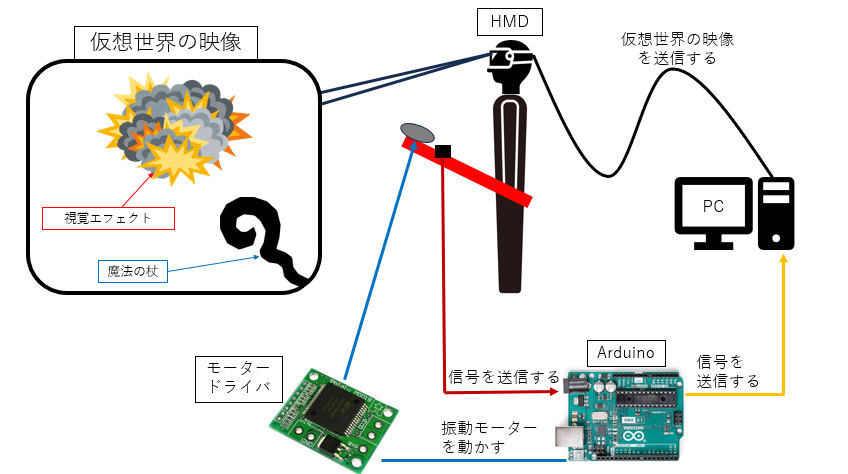
\includegraphics[clip,width=10cm]{fig/systemhard.png}
\caption{システム構成}\label{sys}
\end{figure}

\newpage

\subsection{コントローラー}
上記の構成の中で角材・押しボタン・VIVEトラッカーによってコントローラーを構成している.押しボタンを押すことでArduinoに信号を送る.
Arduinoが信号を受信するとモータードライバに信号を送り振動モーターを回転させ,コントローラ―を振動させる.
\figref{controller}に本システムのコントローラーを示す.

\begin{figure}[h]
\centering
\includegraphics[clip,width=10cm]{./fig/controller.png}
\caption{コントローラー}\label{controller}
\end{figure}





%----------------------------------------------------------------------------------------------

\subsection{ソフトウェアシステム構成}
本研究のシステムに使用したソフトウェアの構成を\tabref{tab;software}に示す.

\begin{table}[H]
    \caption{\label{tab;software}ソフトウェア実装環境}
    \centering
    \begin{tabular}{l|l}
    \hline
    \hline
    OS & Windows 11\\
    開発言語 & C\#\\
    ゲームエンジン & Unity(2021.1.15f1)\\
    \hline
    \end{tabular}
\end{table}

\subsection{視覚エフェクトと振動刺激提示の連動}
前述したコントローラーに装着されている押しボタンを押すとArduinoに信号が送られる.
その信号を受け取ったArduinoからモータードライバとUnityに信号を送信することで視覚エフェクトと振動刺激の提示を連動させている.

\subsection{Unity}
\figref{virtualworld}に開発した仮想世界を示す.

仮想世界には魔法の杖と足場がある.魔法の杖は現実空間のコントローラーの動きと同期している.
コントローラーのボタンを押すと仮想空間上に視覚エフェクトが表示される.
そのときArduinoとシリアル通信を行い振動モーターを回転させる.

\begin{figure}[h]
\centering
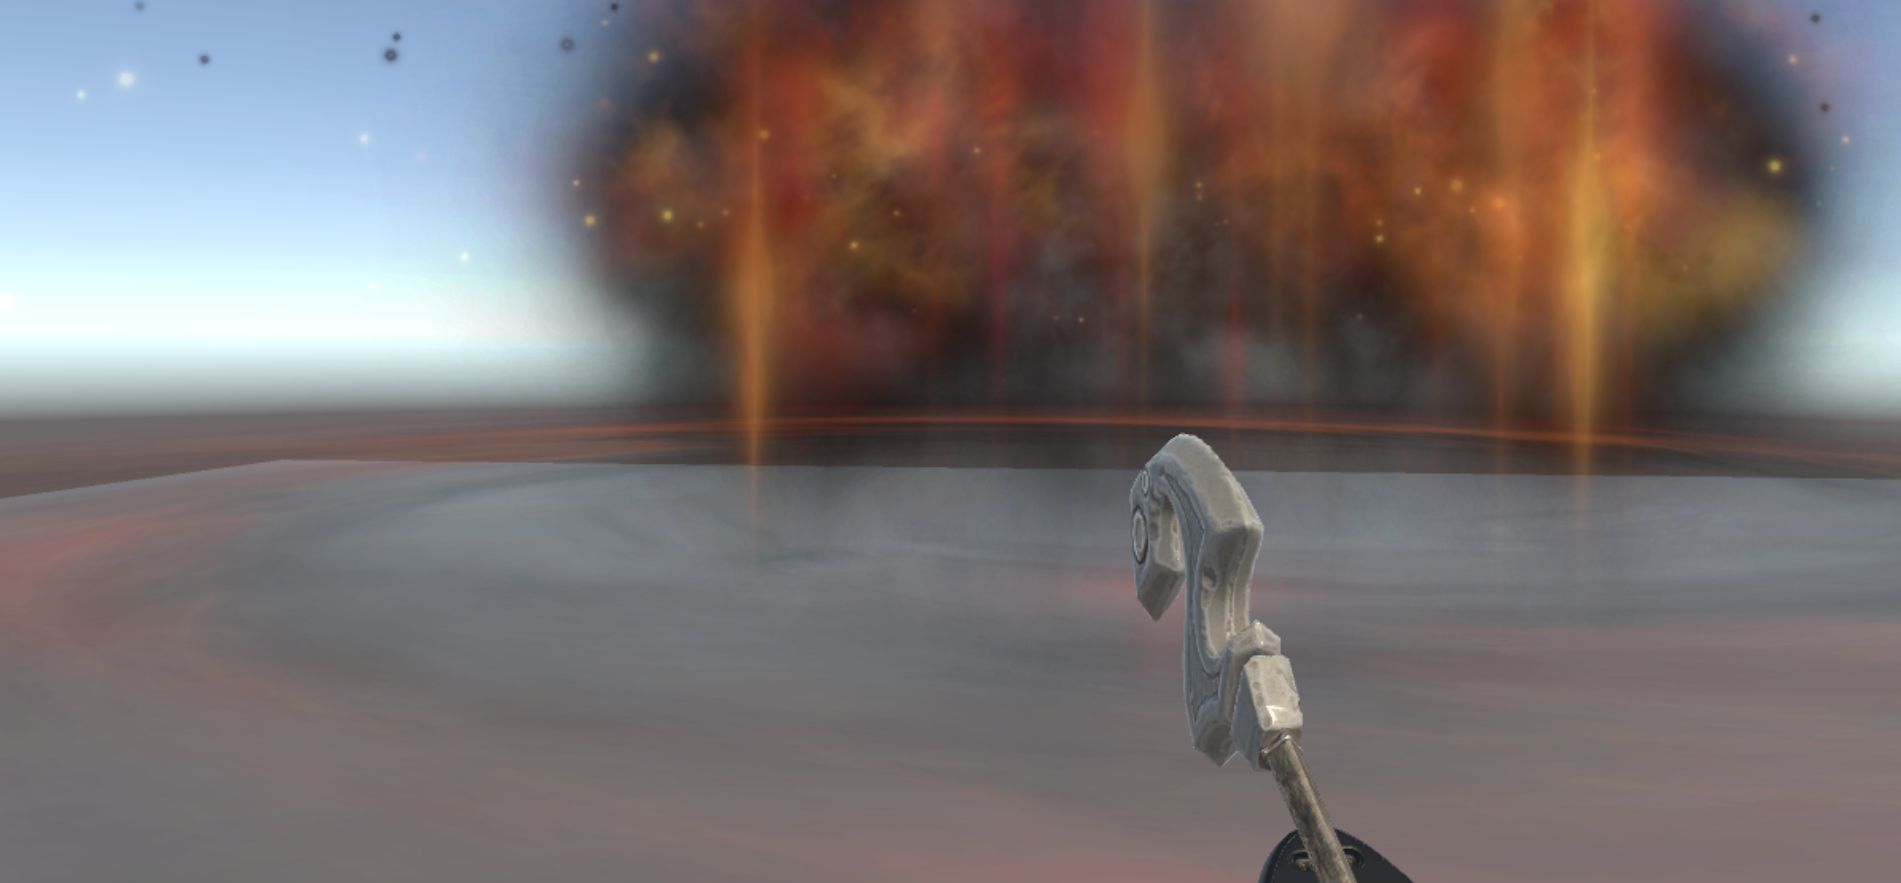
\includegraphics[clip,width=10cm]{fig/unity.png}
\caption{仮想世界}\label{virtualworld}
\end{figure}